\documentclass[report]{IEEEtran}

% *** GRAPHICS RELATED PACKAGES ***
%
\ifCLASSINFOpdf

\usepackage[justification=centering]{caption}
\usepackage{placeins}

   \usepackage[pdftex]{graphicx}
  % declare the path(s) where your graphic files are
  % \graphicspath{{../pdf/}{../jpeg/}}
  % and their extensions so you won't have to specify these with
  % every instance of \includegraphics
  % \DeclareGraphicsExtensions{.pdf,.jpeg,.png}
\else
  % or other class option (dvipsone, dvipdf, if not using dvips). graphicx
  % will default to the driver specified in the system graphics.cfg if no
  % driver is specified.
  % \usepackage[dvips]{graphicx}
  % declare the path(s) where your graphic files are
  % \graphicspath{{../eps/}}
  % and their extensions so you won't have to specify these with
  % every instance of \includegraphics
  % \DeclareGraphicsExtensions{.eps}
\fi
% graphicx was written by David Carlisle and Sebastian Rahtz. It is
% required if you want graphics, photos, etc. graphicx.sty is already
% installed on most LaTeX systems. The latest version and documentation can
% be obtained at: 
% http://www.ctan.org/tex-archive/macros/latex/required/graphics/
% Another good source of documentation is "Using Imported Graphics in
% LaTeX2e" by Keith Reckdahl which can be found as epslatex.ps or
% epslatex.pdf at: http://www.ctan.org/tex-archive/info/
%
% latex, and pdflatex in dvi mode, support graphics in encapsulated
% postscript (.eps) format. pdflatex in pdf mode supports graphics
% in .pdf, .jpeg, .png and .mps (metapost) formats. Users should ensure
% that all non-photo figures use a vector format (.eps, .pdf, .mps) and
% not a bitmapped formats (.jpeg, .png). IEEE frowns on bitmapped formats
% which can result in "jaggedy"/blurry rendering of lines and letters as
% well as large increases in file sizes.
%
% You can find documentation about the pdfTeX application at:
% http://www.tug.org/applications/pdftex








% *** SPECIALIZED LIST PACKAGES ***
%
%\usepackage{algorithmic}
% algorithmic.sty was written by Peter Williams and Rogerio Brito.
% This package provides an algorithmic environment for describing algorithms.
% You can use the algorithmic environment in-text or within a figure
% environment to provide for a floating algorithm. Do NOT use the algorithm
% floating environment provided by algorithm.sty (by the same authors) or
% algorithm2e.sty (by Christophe Fiorio) as IEEE does not use dedicated
% algorithm float types and packages that provide these will not provide
% correct IEEE style captions. The latest version and documentation of
% algorithmic.sty can be obtained at:
% http://www.ctan.org/tex-archive/macros/latex/contrib/algorithms/
% There is also a support site at:
% http://algorithms.berlios.de/index.html
% Also of interest may be the (relatively newer and more customizable)
% algorithmicx.sty package by Szasz Janos:
% http://www.ctan.org/tex-archive/macros/latex/contrib/algorithmicx/





% *** PDF, URL AND HYPERLINK PACKAGES ***
%
%\usepackage{url}
% url.sty was written by Donald Arseneau. It provides better support for
% handling and breaking URLs. url.sty is already installed on most LaTeX
% systems. The latest version can be obtained at:
% http://www.ctan.org/tex-archive/macros/latex/contrib/misc/
% Read the url.sty source comments for usage information. Basically,
% \url{my_url_here}.

% correct bad hyphenation here
%\hyphenation{op-tical net-works semi-conduc-tor}


\begin{document}
%
% paper title
% can use linebreaks \\ within to get better formatting as desired
\title{Shuffleless MapReduce in Go}

% author names and affiliations
% use a multiple column layout for up to three different
% affiliations
\author{\IEEEauthorblockN{Ivan Lugo, Darin Doria, William Adkins, Guy Bean}
\IEEEauthorblockA{\\
ivan.lugo@knights.ucf.edu,
doria@knights.ucf.edu,
wadkins@knights.ucf.edu}}

\thanks{\\Electrical Engineering and Computer Science\\
University of Central Florida\\
Orlando, FL 32816\\}

%
%
% author names and IEEE memberships
% note positions of commas and nonbreaking spaces ( ~ ) LaTeX will not break
% a structure at a ~ so this keeps an author's name from being broken across
% two lines.
% use \thanks{} to gain access to the first footnote area
% a separate \thanks must be used for each paragraph as LaTeX2e's \thanks
% was not built to handle multiple paragraphs
%

%\author{Michael~Shell,~\IEEEmembership{Member,~IEEE,}
 %       John~Doe,~\IEEEmembership{Fellow,~OSA,}
%        and~Jane~Doe,~\IEEEmembership{Life~Fellow,~IEEE}% <-this % stops a space
%\thanks{M. Shell is with the Department
%of Electrical and Computer Engineering, Georgia Institute of Technology, Atlanta,
%GA, 30332 USA e-mail: (see http://www.michaelshell.org/contact.html).}% <-this % stops a space
%\thanks{J. Doe and J. Doe are with Anonymous University.}% <-this % stops a space
%\thanks{Manuscript received April 19, 2005; revised January 11, 2007.}}

% note the % following the last \IEEEmembership and also \thanks - 
% these prevent an unwanted space from occurring between the last author name
% and the end of the author line. i.e., if you had this:
% 
% \author{....lastname \thanks{...} \thanks{...} }
%                     ^------------^------------^----Do not want these spaces!
%
% a space would be appended to the last name and could cause every name on that
% line to be shifted left slightly. This is one of those "LaTeX things". For
% instance, "\textbf{A} \textbf{B}" will typeset as "A B" not "AB". To get
% "AB" then you have to do: "\textbf{A}\textbf{B}"
% \thanks is no different in this regard, so shield the last } of each \thanks
% that ends a line with a % and do not let a space in before the next \thanks.
% Spaces after \IEEEmembership other than the last one are OK (and needed) as
% you are supposed to have spaces between the names. For what it is worth,
% this is a minor point as most people would not even notice if the said evil
% space somehow managed to creep in.



% The paper headers
%\markboth{Journal of \LaTeX\ Class Files,~Vol.~6, No.~1, January~2007}%
%{Shell \MakeLowercase{\textit{et al.}}: Bare Demo of IEEEtran.cls for Journals}
% The only time the second header will appear is for the odd numbered pages
% after the title page when using the twoside option.
% 
% *** Note that you probably will NOT want to include the author's ***
% *** name in the headers of peer review papers.                   ***
% You can use \ifCLASSOPTIONpeerreview for conditional compilation here if
% you desire.




% If you want to put a publisher's ID mark on the page you can do it like
% this:
%\IEEEpubid{0000--0000/00\$00.00~\copyright~2007 IEEE}
% Remember, if you use this you must call \IEEEpubidadjcol in the second
% column for its text to clear the IEEEpubid mark.



% use for special paper notices
%\IEEEspecialpapernotice{(Invited Paper)}




% make the title area
\maketitle

\tableofcontents


\begin{abstract}
%\boldmath
This project involves improving on the classic implementation of MapReduce by executing the  three phases of map reduce as concurrently as the algorithm allows. The goal is to significantly improve the runtime over a sequential implementation running on a shared memory architecture machine. We chose to implement this solution using the Go programming language because it includes built in concurrent primitives that allows us to quickly and effectively write code that can run concurrently, while offloading tedious concepts like locking variable access to the language's runtime environment. The performance results are benchmarked not only against a sequential implementation, but also compared to running on a machine with different amounts of logical processors. Further, we show an example of the overuse of the same primitives available in Go that show a multiplicative increase in runtime.

\end{abstract}

% IEEEtran.cls defaults to using nonbold math in the Abstract.
% This preserves the distinction between vectors and scalars. However,
% if the journal you are submitting to favors bold math in the abstract,
% then you can use LaTeX's standard command \boldmath at the very start
% of the abstract to achieve this. Many IEEE journals frown on math
% in the abstract anyway.

% Note that keywords are not normally used for peerreview papers.
\begin{IEEEkeywords}
IEEEtran, journal, \LaTeX, paper, template.
\end{IEEEkeywords}

\section{Introduction}

\IEEEPARstart {M}{apReduce} is a paradigm, or thought process, in computer programming that is used to process large data sets and convert them into some meaningful information for the computer programmer. The process works by taking several computers, called nodes, and organizing them into a group structure. There are two types of group structures that can be created when linking nodes. The first is a cluster, which is a grouping of nodes that all have similar physical specifications and are on the same local area network. The second is a grid, which is essentially the compliment of a cluster in that the nodes can be made up of many different types of hardware, and can be distributed over a distributed system.
In either model the nodes do the majority of the work, with a main framework machine organizing the movement and distribution of data, data storage, and data back up in the instance of node failures. Each node executes several serial segments of code generally broken down into three phases: the Map phase, the Shuffle phase, and the Reduce phase.

\subsection{Map Phase}
Each node executes a map() function that takes the input data and parses it down into some usable batch of data hence called a token. The node then maps over all the input and creates a token for each user defined chunk. This can be something as simple as a character, or a word, or it can be something much larger and more complicated. Once tokens have been created for each chunk of the input data all the tokens are gathered into a single location for collection into the shuffle phase.

\subsection{Shuffle Phase}
The main framework gathers all of the mapped tokens and redistributes them so that all tokens of like category are sent to a single node. Usually this is done by examining the tokens, which are generally (key, value) pairs, and grouping the tokens by key.

\subsection{Reduce Phase}
Each node then begins executing its reduce() function. This takes all of the tokens and preforms some meaningful work, also user defined, on them in order to turn them into a single updated (key, value) pair. Examples of this can be summing up word counts over a document, calculating different statistics about every user in a website's directory, or even managing a database query. Once all the tokens have been reduced the main framework takes all the reduced values and compiles them into a list to display as the output of the program.

% An example of a floating figure using the graphicx package.
% Note that \label must occur AFTER (or within) \caption.
% For figures, \caption should occur after the \includegraphics.
% Note that IEEEtran v1.7 and later has special internal code that
% is designed to preserve the operation of \label within \caption
% even when the captionsoff option is in effect. However, because
% of issues like this, it may be the safest practice to put all your
% \label just after \caption rather than within \caption{}.
%
% Reminder: the "draftcls" or "draftclsnofoot", not "draft", class
% option should be used if it is desired that the figures are to be
% displayed while in draft mode.
%
%\begin{figure}[!t]
%\centering
%\includegraphics[width=2.5in]{myfigure}
% where an .eps filename suffix will be assumed under latex, 
% and a .pdf suffix will be assumed for pdflatex; or what has been declared
% via \DeclareGraphicsExtensions.
%\caption{Simulation Results}
%\label{fig_sim}
%\end{figure}

% Note that IEEE typically puts floats only at the top, even when this
% results in a large percentage of a column being occupied by floats.


% An example of a double column floating figure using two subfigures.
% (The subfig.sty package must be loaded for this to work.)
% The subfigure \label commands are set within each subfloat command, the
% \label for the overall figure must come after \caption.
% \hfil must be used as a separator to get equal spacing.
% The subfigure.sty package works much the same way, except \subfigure is
% used instead of \subfloat.
%
%\begin{figure*}[!t]
%\centerline{\subfloat[Case I]\includegraphics[width=2.5in]{subfigcase1}%
%\label{fig_first_case}}
%\hfil
%\subfloat[Case II]{\includegraphics[width=2.5in]{subfigcase2}%
%\label{fig_second_case}}}
%\caption{Simulation results}
%\label{fig_sim}
%\end{figure*}
%
% Note that often IEEE papers with subfigures do not employ subfigure
% captions (using the optional argument to \subfloat), but instead will
% reference/describe all of them (a), (b), etc., within the main caption.


% An example of a floating table. Note that, for IEEE style tables, the 
% \caption command should come BEFORE the table. Table text will default to
% \footnotesize as IEEE normally uses this smaller font for tables.
% The \label must come after \caption as always.
%


% Note that IEEE does not put floats in the very first column - or typically
% anywhere on the first page for that matter. Also, in-text middle ("here")
% positioning is not used. Most IEEE journals use top floats exclusively.
% Note that, LaTeX2e, unlike IEEE journals, places footnotes above bottom
% floats. This can be corrected via the \fnbelowfloat command of the
% stfloats package.



\section{GOLANG}

The Go language started as a purely research oriented project in Google Inc.'s Labs, its development headed by Robert Griesemer, Rob Pike, and Ken Thompson in 2007. \cite{FAQ} It was designed around the principles of simplistic and idiomatic concurrency, and done so through the creation of some of its primitive commands and data types: the 'goroutine' method of concurrent execution and its related 'go' command, 'channels' used as blocking and safe interthread communication tools for concurrent data manipulation, and the 'select' command, a switching statement for the aforementioned channels that allows for arbitrary functions or concurrently executing goroutines to quickly and easily choose the most readily available input from a channel.

"Concurrency is not parallelism," \cite{FAQ} is the mainstay of the Go language. This guiding principle states that inherently concurrent challenges should be solved as such, and the realization that a parallel solution is something entirely different drives the underlying primitives. Building on this, the static typing of the language coupled with a modest form of object oriented capabilities helps to ensure that the very model of concurrency Go tries to build is not hampered by unsafe type conversions, memory accesses, or even simple programming errors at compile time.

One of the most fundamentally useful tools prescribed in the language is the goroutine: a construct that may be thought of as a lightweight thread of execution with a small enough footprint to be created in the magnitude of hundreds of thousands with a tiny memory overhead, yet still offering all the runtime benefits of thread scheduling and concurrent execution. Any function declared in Go - including anonymous functions and closures - may be commanded to run in one of these lightweight threads with the use of the prefix 'go'. So long as the program as a whole is capable of handling the concurrency introduced with this prefix, that is all that must be done.

Channels, combined with the concurrency enabled by a goroutine, provides an efficient and safe way for those lightweight threads to communicate with one other. Channels may either be used to receive and send arbitrary blocks of data from and to any goroutine with a reference to the channel and with interest in its contents. Instantiation is done in the same way as any other language level primitive, and once instantiated, may be used indefinitely until it has been closed. The ability to communicate on a channel, while still a nicety, is not its most interesting quality. A channel will block further execution of a goroutine on a send until a receive counterpart has acknowledged the send operation, and likewise, a receive operation will block further execution until a send operation has sent its data and raised a flag. While this is happening, the runtime environment will actually move whichever routine is blocking off of its own thread of execution onto a burner thread, allowing the rest of the program as a whole to continue until that thread is able to continue with its matched channel send or receive. This optimization of execution is something exploited heavily in the implementation discussed, and indeed, one of the most powerful features of lightweight threading. Combining this with the the 'select' statement, a complex structure of handling communication events can 'fan in' from a number of channels and only pop into the main execution thread when it is ready, rather than sitting and spinning on a mutex or lock.

\section{Challenge}
\subsection{Problem Statement}
Map reduce is normally done in three sequential phases. The problem is that each phase depends on the data being received from the previous phase. The process is entirely limited in how fast you can finish by how quickly the previous phase computes all its data and passes it on to the next phase. Current implementations attempt to increase overall speed by computing each phase of data concurrently, whether on a shared memory architecture or across a distributed system of computers, then passing it on to the next phase and repeating those steps until the process completes. The goal of our project is not only to compute each one of these phases concurrently, but to maximize how much of the computing can be done in parallel. There is only so much that can be computed in parallel since, by the very nature of map reduce algorithms, you need all the data from the previous phase before you can proceed. 

\subsection {Why Go?}
Initially the thought of using Go came after researching how previous versions of map-reduce had been implemented. The most notorious version was the one implemented by Google of course. A bit more research led to finding and verifying that google's own programming language is a great fit for map reduce. Go provides built in primitives that allow the language to handle and optimize complex concurrent concepts. This allows us to easily get around common bottlenecks that are introduced when writing multithreaded programs by thinking in a multithreaded fashion without having to explicitly deal with the threads, monitors or locks.

We gain a huge advantage in debugging and programming time by allowing the language to handle threads and locks. The biggest gain is achieved when maximizing the use of goroutines and channels. Passing data through the use of channels helps us get around the use of traditional locks. Because our solution revolves primarily around running several functions concurrently, Go is a perfect fit for the solution. 

\section{Our Solution}

Our implementation on MapReduce focuses on when the user only cares about some subset of the data being searched. The user inputs a list of the key terms in addition to the data to be searched, and we return the values of just those key. While our implementation provides less information that standard MapReduce, it gives us a key advantage. In standard MapReduce, the program doesn't know how many reducers to create until it's finished the shuffle phase, but in our MapReduce, we know we want one reducer per keyword (or maybe some multiple). This knowledge allows us to create map, shuffle, and reduce phases that can run concurrently with each other. We first create our reducers and the channels they receive off of, then create mappers which have access to these channels and can thus communicate with the reducers directly. The shuffle phase then becomes an implicit part of the map phase, while the reduce phase is simply receiving a stream of data from mappers as they finish. This extra concurrency, we propose, will speed up runtime, even when the worst case runtime of our phases is the same as the standard implementation. 

We start by taking in the files our user wants to search and the keywords they care about. We create the reducers and channels for those keywords, and set them to run in goroutines. We then create a mapper for each input file, each with the ability to send data across each of the reducer channels. They then iterate through their assigned input, hashing each word and incrementing the index of the result. This means the mapping phase has a runtime of O(n), where n is the number of words in the input file.

When a mapper finds the end of their input, they send the keyword's counts through the appropriate channels to their corresponding reducer. They then send a flag back to main, which is used in judging when to call for the final results. This phase has a runtime of O(m), where m is the number of keywords the user input.

The reducers each keep a running total of the data points they have received. They treat their channel like a queue; constantly popping values and adding them to their total. If their channel is emptied, they must wait for further instruction. The channels will be closed when all mappers are done, until that point no reducer can be guaranteed to have a correct final result, as any mapper's completion can affect all reducers result. The reducers each have buffer size limit on their channel, and are nonblocking until their buffer is filled. When main receives a flag from every mapper, it closes the receiver's channels and starts listening for results. Any receiver that is already done will send its final result across another channel to main, which will output data as it receives it. Reducers that are not done will continue to compute until emptying out their channel, and send their final result to main as they finish. The reducers have a runtime of O(k), where k is the number of mappers created, as each mapper can only send data to any given reducer once.

\section{Results}
See ExecutionComparison.
[Preliminary]

\begin{figure}[h]
\centering
	
\includegraphics[width = 8.75cm]{image2}
	\caption{A Lovley Image}
		
\end{figure}

\begin{figure}[h]
\centering
	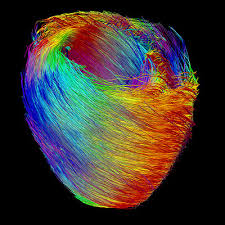
\includegraphics[width = 8.75cm]{image1}
	\caption{A Lovley Image}
		
\end{figure}

\begin{figure}[h]
\centering
	
\includegraphics[width = 8.75cm]{image2}
	\caption{A Lovley Image}
		
\end{figure}

\begin{figure}[h]
\centering
	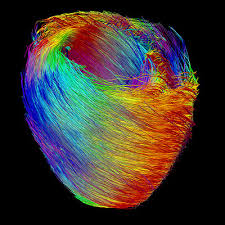
\includegraphics[width = 8.75cm]{image1}
	\caption{A Lovley Image}
		
\end{figure}

\begin{figure}[h]
\centering
	
\includegraphics[width = 8.75cm]{image2}
	\caption{A Lovley Image}
		
\end{figure}

\begin{figure}[h]
\centering
	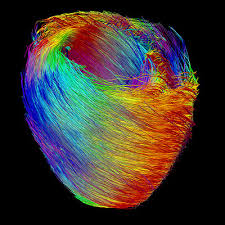
\includegraphics[width = 8.75cm]{image1}
	\caption{A Lovley Image}
		
\end{figure}



%\begin{table}[!t]
%% increase table row spacing, adjust to taste
%\renewcommand{\arraystretch}{1.3}
% if using array.sty, it might be a good idea to tweak the value of
% \extrarowheight as needed to properly center the text within the cells
%\caption{Overall Execution Comparison [v1]}
%\label{ExecutionComparison}
%\centering
%% Some packages, such as MDW tools, offer better commands for making tables
%% than the plain LaTeX2e tabular which is used here.

%\begin{tabular}{|c||c||c||c|}
%\hline
%File Count & Parallel & Sequential & 1.x Delta\\
%\hline
%32 Files & 1.909212533 & 2.6275413 & 1.37624348\\
%\hline
%64 Files & 3.682723233 & 5.158865333 & 1.400828954\\
%\hline
%128 Files & 7.283922367 & 10.2794731 & 1.41125517\\
%\hline
%256 Files & 14.33229347 & 20.5493898 & 1.433782377\\
%\hline
%512 Files & 28.83089667 & 41.0223975 & 1.422862354\\
%\hline
%1024 Files & 55.89146183 & 81.83026183 & 1.464092352\\
%\hline
%2048 Files & 111.1820113 & 162.9768163 & 1.465855981\\
%\hline
%4096 Files & 222.8098348 & 329.5016414 & 1.478846935\\
%\hline
%\end{tabular}
%\end{table}

\FloatBarrier

\section{Conclusion}
[To be written for final report.]

\section{Future Work}

There are a few potential optimizations and utilities we found that might improve upon our algorithm. One potential optimization would be to generate multiple reducers per word, instead of only one. This would allow for effectively larger channel buffers, as when a channel fills its buffer it blocks until room is created. It could also be expanded into dynamically resizing reducers, where more reducers are created for a word when its buffer fills. The potential pitfalls of this would involve each word needing a reducer hub or controller, to manage the reducers for a word, distribute incoming tokens, and merge the results when all reducers are done. This could cause bottlenecking; as every request would go through the hub to be distributed across the multiple reducers for a word. Additionally, it would add another level of blocking to the end of the algorithm; each reducer hub would need to block sending its results until every one of its reducers returned a value. A potential utility to expand on our algorithm would be the creation of a generic framework that could take in a map and reduce function from the user and use our algorithm in conjunction with these functions to derive an answer to whatever question. This might slow down the algorithm, as doing so would require changing our mapping logic to operate on the output of the supplied mapping logic, instead of processing the data as its iterated through.


% if have a single appendix:
%\appendix[Proof of the Zonklar Equations]
% or
%\appendix  % for no appendix heading
% do not use \section anymore after \appendix, only \section*
% is possibly needed

% use appendices with more than one appendix
% then use \section to start each appendix
% you must declare a \section before using any
% \subsection or using \label (\appendices by itself
% starts a section numbered zero.)
%


%\appendix
%\section*{Foreseeable Issues}
%	\begin{itemize}
%		\item Determining how to distribute work loads amongst any arbitrary amount of workers is very tricky. It has to be dynamically calculated and will change depending on the size of the total input being mapped. This step is crucial as it affects the outcome of the program?s overall %performance. Spawning too many mappers can result in too much overhead without getting enough return in speed to make up for it. On the other hand, not creating enough mappers means that the few mappers doing work might not be able to compute and output data fast enough to have the %reducers constantly consuming.
%		\item Setting `runtime.GOMAXPROCS()` can backfire and potentially negatively impact overall program execution. Keep in mind that Go?s native functionality is built for concurrency, which is not the same as parallelism. When increasing the amount of logical processors it allows the %program?s goroutines to be run in parallel across multiple logical processors, but this is not always a good thing or what the programmer expects. At that point the Go language does not have the same power of interleaving goroutines as it usually does on one processor. This can lead to %goroutines  finishing before expected. If this thought is not kept in mind when writing the program the results can either be completely different every time or slow down the performance time.
%		\item A solution to appropriately splitting up the work may be to call mappers and reducers recursively. Implementing it this way means that it collides with the end goal of creating a generic framework because we would have to modify the user?s code, but that does not mean that it %cannot be done.
%		\item To achieve non-blocking execution across multiple goroutines we must use buffered channels. After the channel meets the buffer limit it will block the same way a traditional channel blocks. The use of buffered channels requires careful thought of where they are used and how much %of a buffer limit is set, if not, it will also lead to unexpected results.
%	\end{itemize}
%\section*{Completed Work}
%	\begin{itemize}
%		\item Built proof of concept using built in Go concurrent primitives and following common Go practices.
%		\item Compare and benchmark against an alternate sequential implementation.
%		\item Use the sequential implementation as a base benchmark for future improvements.
%	\end{itemize}

%\section*{Incomplete Work}
%	\begin{itemize}
%		\item Create a general framework that allows a user to write their own map and reduce functions based on a specified input.
%		\item Make the framework non blocking so each phase of the map-reduce process can perform computations in parallel.
%	\end{itemize}

% Can use something like this to put references on a page
% by themselves when using endfloat and the captionsoff option.
%\ifCLASSOPTIONcaptionsoff
%  \newpage
%\fi



% trigger a \newpage just before the given reference
% number - used to balance the columns on the last page
% adjust value as needed - may need to be readjusted if
% the document is modified later
%\IEEEtriggeratref{8}
% The "triggered" command can be changed if desired:
%\IEEEtriggercmd{\enlargethispage{-5in}}

% references section

% can use a bibliography generated by BibTeX as a .bbl file
% BibTeX documentation can be easily obtained at:
% http://www.ctan.org/tex-archive/biblio/bibtex/contrib/doc/
% The IEEEtran BibTeX style support page is at:
% http://www.michaelshell.org/tex/ieeetran/bibtex/
%\bibliographystyle{IEEEtran}
% argument is your BibTeX string definitions and bibliography database(s)
%\bibliography{IEEEabrv,../bib/paper}
%
% <OR> manually copy in the resultant .bbl file
% set second argument of \begin to the number of references
% (used to reserve space for the reference number labels box)
\begin{thebibliography}{9}

\bibitem{FAQ}
"Frequently Asked Questions (FAQ)." - The Go Programming Language. 
February 4, 2015. Accessed March 25, 2015. http://golang.org/doc/faq.

\bibitem{DATA}
"Tool: Random String Generator [Test Data Creation]." Random String Generator. 
Accessed March 25, 2015. http://textmechanic.com/Random-String-Generator.html.

\bibitem{BAN}
Bravendar, Dan. "MapReduce for Go." MapReduce for Go. November 24, 2009. 
Accessed March 25, 2015. http://dan.bravender.net/2009/11/24/MapReduce\_for\_Go.html.

\bibitem{ORIGIN}
Dean, Jeffrey, and Sanjay Ghemawat. MapReduce: Simplified Data Processing on Large Clusters. OSDI, 2014.

\end{thebibliography}


% biography section
% 
% If you have an EPS/PDF photo (graphicx package needed) extra braces are
% needed around the contents of the optional argument to biography to prevent
% the LaTeX parser from getting confused when it sees the complicated
% \includegraphics command within an optional argument. (You could create
% your own custom macro containing the \includegraphics command to make things
% simpler here.)
%\begin{biography}[{\includegraphics[width=1in,height=1.25in,clip,keepaspectratio]{mshell}}]{Michael Shell}
% or if you just want to reserve a space for a photo:

%\begin{IEEEbiography}{Michael Shell}
%Biography text here.
%\end{IEEEbiography}

% if you will not have a photo at all:
%\begin{IEEEbiographynophoto}{John Doe}
%Biography text here.
%\end{IEEEbiographynophoto}

% insert where needed to balance the two columns on the last page with
% biographies
%\newpage

%\begin{IEEEbiographynophoto}{Jane Doe}
%Biography text here.
%\end{IEEEbiographynophoto}

% You can push biographies down or up by placing
% a \vfill before or after them. The appropriate
% use of \vfill depends on what kind of text is
% on the last page and whether or not the columns
% are being equalized.

%\vfill

% Can be used to pull up biographies so that the bottom of the last one
% is flush with the other column.
%\enlargethispage{-5in}



% that's all folks
\end{document}


